\documentclass[12pt,a4paper]{book}
\raggedbottom

\usepackage{ugmath}
\usepackage{float}
\usepackage{placeins}
\usepackage[labelfont=bf,labelsep=space]{caption}
\usepackage{pdfpages}
\usepackage{tikz-cd}
\usepackage{amsthm}
\DeclareMathOperator{\rg}{rg}
\renewcommand{\Tr}{\operatorname{Tr}}
\newcommand{\llaves}[1]{\{#1\}}
\newcommand{\parentesis}[1]{\left(#1\right)}
\newcommand{\corchetes}[1]{\left[#1\right]}
\newcommand{\llavesgrande}[1]{\big\{#1\big\}}
\newcommand{\llavesgrandes}[1]{\left\{#1\right\}}


\begin{document}
    
    
    \thispagestyle{empty}
    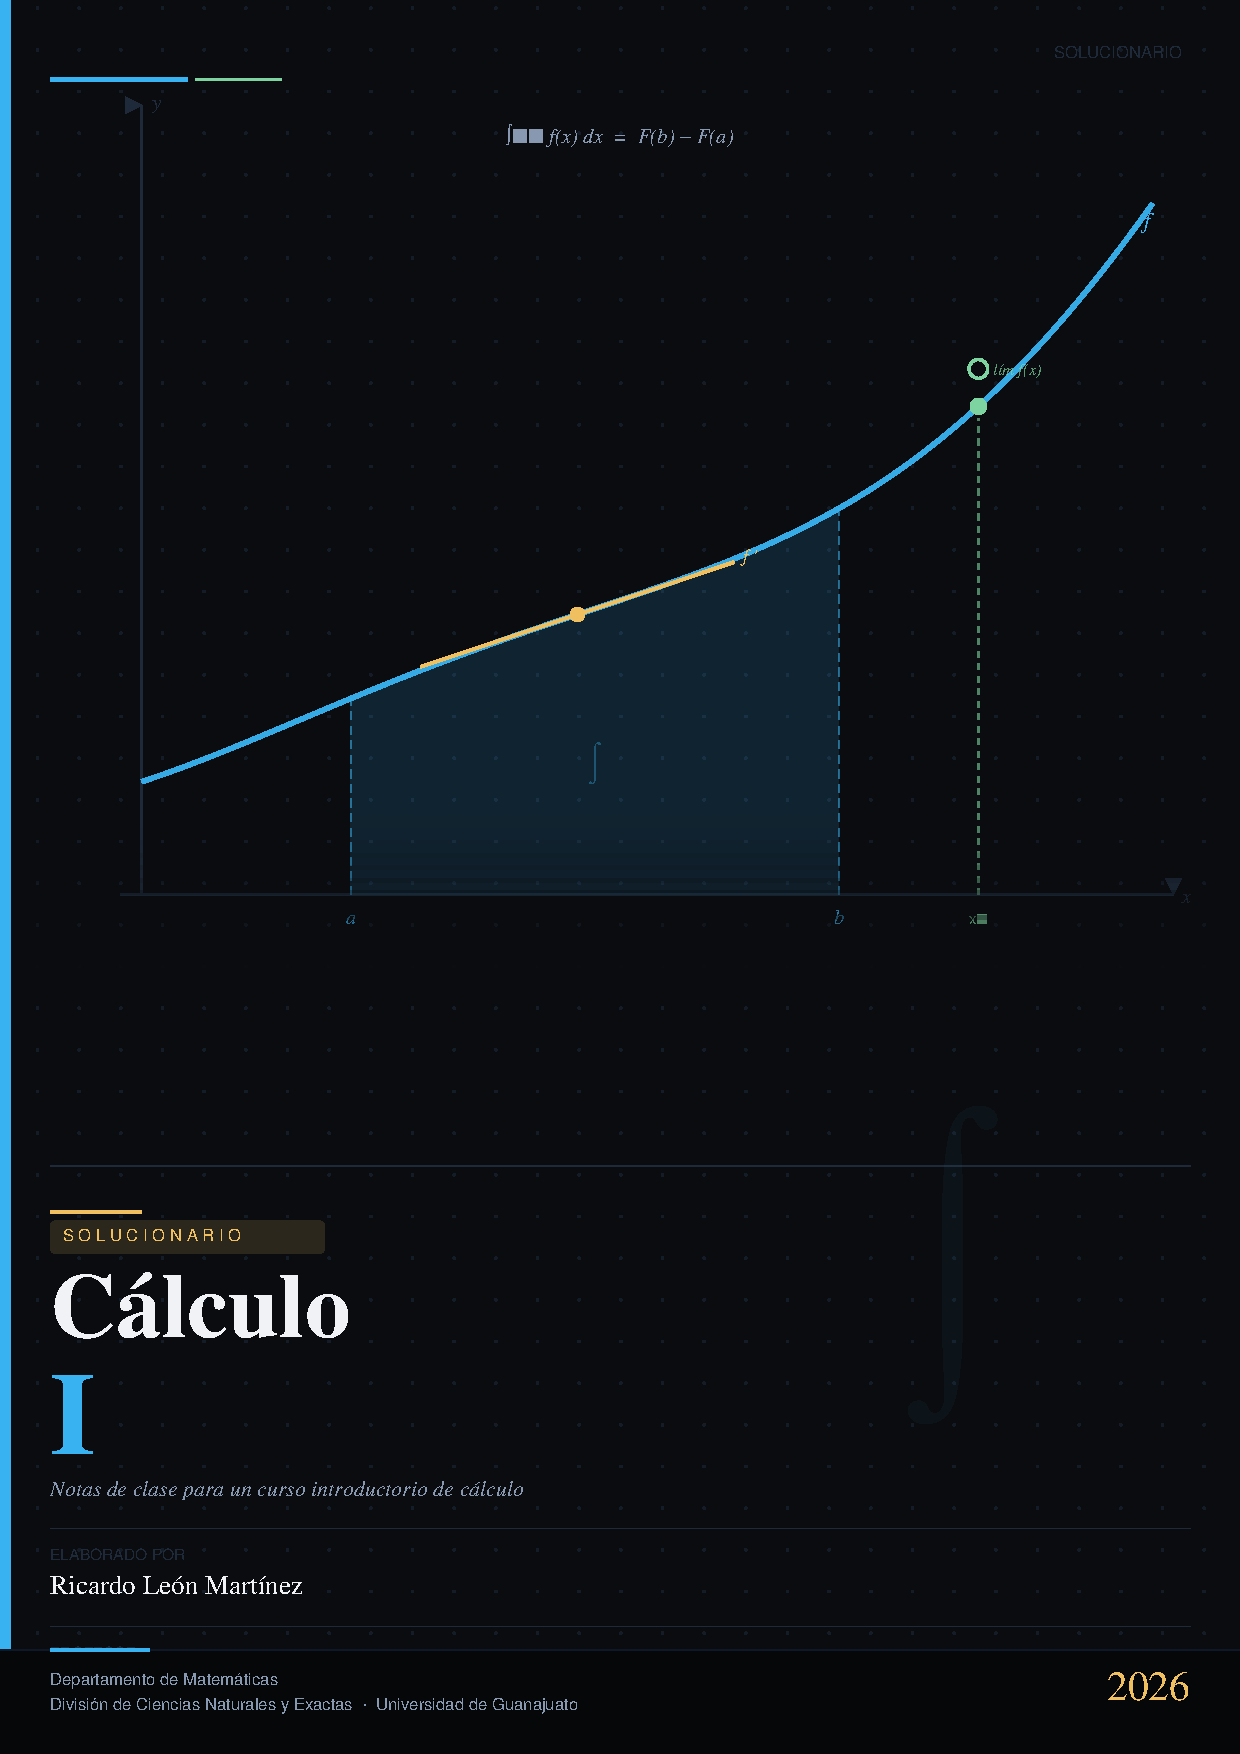
\includepdf[pages=1]{portada_solucionario_calculo1.pdf}

    \begin{flushright}
      \thispagestyle{empty}

        \textit{Dedicado a sam, por que es mi mejor amiga\\
        y siempre a estado ahi para mi. Dedicado a Kaori que\\
        es tmb mi mejor amiga y que compartimos el sufrimiento\\
        de cursar carreras de ciencias puras.}\\[1cm]

        \textit{La neta estas lo hago para estudiar en vacaciones\\
        y prepararme para recursarla y entenderla bien.}\\[1.2cm]

    \end{flushright}

    % ---------------- NOTA DE ERRORES ----------------

    \cleardoublepage
    \thispagestyle{empty}

    \begin{mdframed}[style=mdgreenbox]
        \begin{center}
        \small
        Este solucionario fue elaborado con fines académicos.\\
        A pesar del cuidado puesto en su redacción,\\
        es posible que existan errores u omisiones.\\[0.3cm]

        Cualquier corrección, sugerencia o comentario será bienvenido
        en los correos: \\[0.3cm]

        
        ricardo.leon@cimat.mx
        \end{center}
    \end{mdframed}

    % -------------------------------------------------
    
    \setcounter{page}{1}
    \tableofcontents

    \chapter{Teoría Intuitiva de Conjuntos}

    \section{Introducción}

    \begin{ejercicio}
        Prueba que el conjunto vacío es el único conjunto sin elementos.
    \end{ejercicio}

    \begin{proof}
        Supongamos que $A$ es un conjunto sin elementos. Entonces para toda $x$, $x\notin A$.
        Para probar que $A\subseteq\varnothing$, sea $x\in A$. Esto es imposible, pues $A$ no tiene
        elementos. Luego la implicación
        \begin{equation*}
            x\in A\implies x\in\varnothing
        \end{equation*}
        es verdadera para todo $x$, y por lo tanto $A\subseteq\varnothing$. Por la proposición 1,
        $\varnothing\subseteq A$. En consecuencia, por el criterio de la igualadad de conjuntos $A=\varnothing$.
        Por lo tanto, el conjunto vacío es único.
    \end{proof}

    \section{Notación de Conjuntos Mediante una Condición}

    \begin{ejercicio}
        Expresa los conjuntos siguientes mediante alguna condición.
        \begin{multicols}{2}
            \begin{enumerate}
                \item[(a)] $\{1,3,5,7,\dots\}$.
                \item[(b)] $\{2,4,6,8,\dots\}$.
                \item[(c)] $\{9,10,11,12,\dots\}$.
                \item[(d)] $\{7,8,\dots,93,94\}$.
                \item[(e)] $\{1,2,4,8,16,\dots\}$.
                \item[(f)] $\{1,1/2,1/3,1/4,\dots\}$.   
            \end{enumerate}
        \end{multicols}
    \end{ejercicio}

    \begin{solucion}
        \begin{multicols}{2}
            \begin{enumerate}
            \item[(a)] $\{1,3,5,7,\dots\}=\{2n-1:n\in\N\}$.
            \item[(b)] $\{2,4,6,8,\dots\}=\{2n:n\in\N\}$.
            \item[(c)] $\{9,10,11,12,\dots\}=\{n\in\N: n\geq9\}$.
            \item[(d)] $\{7,8,\dots,93,94\}=\{n\in\N:7\leq n\leq94\}$.
            \item[(e)] $\{1,2,4,8,16,\dots\}=\{2^{n}:n\in\N\cup\{0\}\}$.
            \item[(f)] $\{1,1/2,1/3,1/4,\dots\}=\left\{\frac{1}{n}:n\in\N\right\}$.  
            \end{enumerate}            
        \end{multicols}
    \end{solucion}

    \begin{ejercicio}
        Prueba que
        \begin{equation*}
            \{x:x\notin x\}
        \end{equation*}
        no es un conjunto. \textbf{Sugerencia:} Procede por contradicción, supón que $A:=\{x:x\notin x\}$
        es un conjunto y considera los casos en que $A\in A$ y $A\notin A$
    \end{ejercicio}

    \begin{proof}
        Supongamos, por contradicción, que
        \begin{equation*}
            A:=\{x:x\notin x\}
        \end{equation*}
        es un conjunto. Por definición de $A$,
        \begin{equation*}
            x\in A\ssi x\notin x.
        \end{equation*}
        En particular, tomando $x=A$, obtenemos
        \begin{equation*}
            A\in A\ssi A\notin A.
        \end{equation*}
        Ahora analizamos los dos casos posibles. Primer caso $A\in A$. Como $A\in A$ y los elementos de
        $A$ son precisamente los conjuntos no pertenecen a si mismos, se sigue que
        \begin{equation*}
            A\notin A
        \end{equation*}
        lo cual contradice la hipótesis $A\in A$. Segundo caso $A\notin A$. Como $A$ no pertenece a su mismo,
        satisface la propiedad que define a los elementos de $A$. Por tanto,
        \begin{equation*}
            A\in A,
        \end{equation*}
        lo cual contradice la hipótesis de $A\notin A$. En ambos casos llegamos a una contradicción.
        Luego nuestra suposición inicial era falsa. Por consiguiente,
        \begin{equation*}
            \{x:x\notin x\}
        \end{equation*}
        no es un conjunto.
    \end{proof}

    \vspace{1cm}

    \section{Operaciones con Conjuntos}

    \begin{ejercicio}
        Sean $A=\{0,1,2,3,4,5,6,7,8,9\}$, $B=\{5,6,7,8,9\}$, $C=\{0,1,2,3,4\}$, $D=\{3,4,5\}$ y
        $E=\{a,e,i,o,u\}$ y $F=\{a,e,o\}$. Calcula lo siguiente:
        \begin{multicols}{2}
            \begin{enumerate}
                \item[(a)] $A\cup B$, $B\cup C$ y $D\cup F$.
                \item[(b)] $A\cap B$, $B\cap C$ y $D\cap F$. 
                \item[(c)] $B\cup C\cup D$ y $B\cap C\cap D$.
                \item[(d)] $B\cup D\cup E$ y $B\cap D\cap E$.
                \item[(e)] $A\setminus B$, $B\setminus A$, $B\setminus C$ y $A\setminus D$.  
                \item[(f)] $A\setminus E$, $E\setminus A$, $E\setminus F$ y $F\setminus E$. 
            \end{enumerate}
        \end{multicols}
    \end{ejercicio}

    \begin{solucion}
        \begin{enumerate}
            \item[(a)] $A\cup B$, $B\cup C$ y $D\cup F$.
            \begin{equation*}
                A\cup B=\{0,1,2,3,4,5,6,7,8,9\},\quad B\cup C=\{0,1,2,3,4,5,6,7,8,9\},\quad D\cup F=\{3,4,5,a,e,o\}.
            \end{equation*}
            \item[(b)] $A\cap B$, $B\cap C$ y $D\cap F$.
            \begin{equation*}
                A\cap B=\{5,6,7,8,9\},\quad B\cap C=\varnothing,\quad D\cap F=\varnothing.
            \end{equation*}
            \item[(c)] $B\cup C\cup D$ y $B\cap C\cap D$.
            \begin{equation*}
                B\cup C\cup D=\{0,1,2,3,4,5,6,7,8,9\},\quad B\cap C\cap D=\varnothing.
            \end{equation*}
            \item[(d)] $B\cup D\cup E$ y $B\cap D\cap E$.
            \begin{equation*}
                B\cup D\cup E=\{3,4,5,6,7,8,9,a,e,i,o,u\},\quad B\cap D\cap E=\varnothing
            \end{equation*}
            \item[(e)] $A\setminus B$, $B\setminus A$, $B\setminus C$ y $A\setminus D$.
            \begin{equation*}
                A\setminus B=\{0,1,2,3,4\},\quad B\setminus A=\varnothing,\quad B\setminus C=\{5,6,7,8,9\},\quad A\setminus D=\{0,1,2,6,7,8,9\}
            \end{equation*}
            \item[(f)] $A\setminus E$, $E\setminus A$, $E\setminus F$ y $F\setminus E$.
            \begin{equation*}
                A\setminus E=\{0,1,2,3,4,5,6,7,8,9\},\quad E\setminus A=\{a,e,i,o,u\},\quad E\setminus F=\{i,u\},\quad F\setminus E=\varnothing
            \end{equation*}
        \end{enumerate}
    \end{solucion}

    \begin{ejercicio}
        Encuentra $\bigcup_{n=1}^{\infty}A_{n}$ y $\bigcap_{n=1}^{\infty}A_{n}$ si $A_{n}=\{1,2,\dots,n\}$
        para cada $n\in\N$.
    \end{ejercicio}
    
    \begin{proof}
        Sea $x\in\bigcup_{n=1}^{\infty}A_{n}$. Por definición de la unión, existe $n\in\N$ tal que $x\in A_{n}$.
        Como
        \begin{equation*}
            A_{n}=\{1,2,\dots,n\},
        \end{equation*}
        se sigue que $x$ es uno de los números $1,2,\dots,n$. En particular, $x\in\N$. Por lo tanto
        \begin{equation*}
            \bigcup_{n=1}^{\infty}A_{n}\subseteq\N.
        \end{equation*}
        Sea $x\in\N$. Tomemos $n=x$. Entonces
        \begin{equation*}
            A_{x}=\{1,2,\dots,x\}.
        \end{equation*}
        Claramente $x\in A_{x}$. Por definición de unión,
        \begin{equation*}
            x\in\bigcup_{n=1}^{\infty}A_{n}.
        \end{equation*}
        Por consiguiente,
        \begin{equation*}
            \N\subseteq\bigcup_{n=1}^{\infty}A_{n}.
        \end{equation*}
        Concluimos que
        \begin{equation*}
            \bigcup_{n=1}^{\infty}A_{n}=\N.
        \end{equation*}
        Sea
        \begin{equation*}
            x\in\bigcap_{n=1}^{\infty}A_{n}.
        \end{equation*}
        Por definición de intersección, $x\in A_{n}$ para todo $n\in\N$. En particular, tomando $n=1$,
        \begin{equation*}
            x\in A_{1}=\{1\}.
        \end{equation*}
        Luego $x=1$. Por tanto,
        \begin{equation*}
            \bigcap_{n=1}^{\infty}A_{n}\subseteq\{1\}.
        \end{equation*}
        Sea $x=1$. Para todo $n\in\N$,
        \begin{equation*}
            1\in A_{n}=\{1,2,\dots\}.
        \end{equation*}
        Por definición de intersección,
        \begin{equation*}
            1\in\bigcap_{n=1}^{\infty}A_{n}.
        \end{equation*}
        Así,
        \begin{equation*}
            \{1\}\in\bigcap_{n=1}^{\infty}A_{n}.
        \end{equation*}
        Concluimos que
        \begin{equation*}
            \bigcap_{n=1}^{\infty}A_{n}=\{1\}.
        \end{equation*}
    \end{proof}

    \begin{ejercicio}
        Encuentra $\bigcup_{n=1}^{\infty}A_{n}$ y $\bigcap_{n=1}^{\infty}A_{n}$ si $A_{n}=\{n,n+1,n+2,\dots\}$
        para cada $n\in\N$.
    \end{ejercicio}

    \begin{proof}
        Sea $x\in\bigcup_{n=1}^{\infty}A_{n}$, entonces $x\in A$ para algún $n$, luego $x\in\N$. Así,
        \begin{equation*}
            \bigcup_{n=1}^{\infty}A_{n}\subseteq\N.
        \end{equation*}
        Si $x\in\N$, entonces $x\in A_{1}$, así que $x\in\bigcup_{n=1}^{\infty}A_{n}$. Así,
        \begin{equation*}
            \N\subseteq\bigcup_{n=1}^{\infty}A_{n}.
        \end{equation*}
        Concluimos que
        \begin{equation*}
            \bigcup_{n=1}^{\infty}A_{n}=\N.
        \end{equation*}
        Sea $x\in\bigcap_{n=1}^{\infty}A_{n}$. Entonces $x\in A_{n}$, $\forall n\in\N$. Como $x\in A_{n}$
        significa $x\geq n$, tendriamos
        \begin{equation*}
            x\geq n\quad\forall n\in\N.
        \end{equation*} 
        Pero esto es imposible, pues tomando $n=x+1$,
        \begin{equation*}
            x\geq x+1,
        \end{equation*}
        contradicción. Así, no existe tal $x$, y por lo tanto
        \begin{equation*}
            \bigcap_{n=1}^{\infty}A_{n}=\varnothing.
        \end{equation*}
    \end{proof}

    \begin{ejercicio}
        Muestra un par de conjuntos $A$ y $B$ tales que $A\times B\neq B\times A$.
    \end{ejercicio}

    \begin{solucion}
        Sea $A=\{1,2\}$ y $B=\{3\}$. Entonces,
        \begin{equation*}
            A\times B=\{(1,3),(2,3)\},\qquad B\times A=\{(3,1),(3,2)\}.
        \end{equation*}
        Así,
        \begin{equation*}
            A\times B\neq B\times A.
        \end{equation*}
    \end{solucion}

    \begin{ejercicio}
        Prueba los incisos (b), (c) y (d) de la proposición 2.
    \end{ejercicio}

    \begin{proof}
        \begin{enumerate}
            \item[(b)] De la serie de implicaciones
            \begin{align*}
                x\in A\cup(B\cup C)&\implies x\in A\lor(x\in B\lor x\in C)\\
                &\implies (x\in A\lor x\in B)\lor x\in C\\
                &\implies x\in(A\cup B)\cup C
            \end{align*}
            obtenemos que $A\cup(B\cup C)\subseteq (A\cup B)\cup C$. Es fácil ver que las implicaciones
            que aparecen también se cumplen en el sentido contrario, de lo cual obtenemos que $(A\cup B)\cup C\subseteq A\cup(B\cup C)$
            y, en consecuencia, que $A\cup(B\cup C)=(A\cup B)\cup C$. La prueba de que $A\cap(B\cap C)=(A\cap B)\cap C$
            es similar.
            \item[(c)] De la serie de implicaciones
            \begin{align*}
                x\in A\cup(B\cap C)&\implies x\in A\lor(x\in B\wedge x\in C)\\
                &\implies (x\in A\lor x\in B)\wedge(x\in A\lor x\in C)\\
                &\implies x\in (A\cup B)\cap(A\cup C)
            \end{align*}
            obtenemos que $A\cup(B\cap C)\subseteq (A\cup B)\cap(A\cup C)$. Es fácil ver que las implicaciones
            que aparecen también se cumplen en el sentido contrario, de lo cual obtenemos $(A\cup B)\cap(A\cup C)\subseteq A\cup(B\cap C)$ y,
            en consecuencia, que $A\cup(B\cap C)=(A\cup B)\cap(A\cup C)$. La prueba de que $A\cap(B\cup C)=(A\cap B)\cup(A\cap C)$ es
            similar.
            \item[(d)] De la serie de implicaciones
            \begin{align*}
                x\in A\setminus(B\cup C)&\implies x\in A \wedge x\notin(B\cup C)\\
                &\implies x\in A\wedge(x\notin B\lor x\notin C)\\
                &\implies (x\in A\wedge x\notin B)\lor (x\in A\wedge x\notin C)\\
                &\implies x\in (A\setminus B)\cup(A\setminus C)
            \end{align*}
            obtenemos que $A\setminus(B\cup C)\subseteq(A\setminus B)\cup(A\setminus C)$. Es fácil ver que las implicaciones
            que aparecen también se cumplen en el sentido horario, de lo cual obtenemos $(A\setminus B)\cup(A\setminus C)\subseteq A\setminus(B\cup C)$
            y, en consecuencia, que $A\setminus(B\cup C)=(A\setminus B)\cup(A\setminus C)$. La prueba de que $A\setminus(B\cap C)=(A\setminus B)\cup(A\setminus C)$
            es similar.
        \end{enumerate}
    \end{proof}

    \begin{ejercicio}
        Prueba la proposición 3
    \end{ejercicio}

    \begin{proof}
        \begin{enumerate}
            \item[(a)] De la serie de implicaciones
            \begin{align*}
                x\in A\cup\varnothing&\implies x\in A\lor x\in\varnothing\\
                &\implies x\in A
            \end{align*}
            obtenemos que $A\cup\varnothing\subseteq A$. Si $x\in A$ por definción es claro que $x\in A\cup\varnothing$.
            En consecuencia $A\subseteq A\cup\varnothing$ y, por lo tanto,
            \begin{equation*}
                A\cup\varnothing=A.
            \end{equation*}
            Sea ahora $x\in A\cap\varnothing$.
            Entonces, por definición de intersección, $x\in A$ y $x\in\varnothing$. Pero $x\in\varnothing$ es imposible,
            ya que el conjunto vacío no tiene elementos. Por lo tanto, no existe ningún $x$ tal que $x\in A\cap\varnothing$.
            En consecuencia, $A\cap\varnothing$ no tiene elementos, es decir,
            \begin{equation*}
                A\cap\varnothing=\varnothing.
            \end{equation*}
            De la serie de implicaciones,
            \begin{align*}
                x\in A\setminus\varnothing&\implies x\in A\wedge x\notin\varnothing\\
                &\implies x\in A
            \end{align*}
            obtenemos que $A\setminus\varnothing\subseteq A$. Si $x\in A$ por definición es claro que
            $x\in A\setminus\varnothing$ y, en consecuencia, $A\subseteq A\setminus\varnothing$. Por lo
            tanto
            \begin{equation*}
                A\setminus\varnothing=A.
            \end{equation*}
            Sea $x\in \varnothing\setminus A$. Entonces por definición de diferencia de conjuntos, $x\in\varnothing\wedge x\notin A$.
            Pero $x\in\varnothing$ es imposible, ya que el conjunto vacío no tiene elementos. Por lo tanto,
            no existe ningún $x$ tal que $x\in \varnothing\setminus A$. En consecuencia, $\varnothing\setminus A$
            no tiene elementos, es decir,
            \begin{equation*}
                \varnothing\setminus A=\varnothing.
            \end{equation*}
            \item[(b)] Si $x\in A\cup B$ entonces $x\in A$ y como $A\subseteq B$ se tiene que $x\in B$ y, por lo tanto
            $A\cup B\subseteq B$. Ahora si $x\in B$ entonces como $A\subseteq B$, obtenemos $x\in A$ y por definición de unión
            $x\in A\cup B$, por consiguiente $B\subseteq A\cup B$. Concluimos que,
            \begin{equation*}
                A\cup B=B.
            \end{equation*}
            Si $x\in A\cap B$ entonces por definición de intersección $x\in A$ y, por tanto $A\cap B\subseteq A$. Ahora si $x\in A$ entonces como $A\subseteq B$
            tenemos que $x\in B$ y por definición de intersección $x\in A\cap B$, y asi, $A\subseteq A\cap B$.
            Concluimos que
            \begin{equation*}
                A\cap B=A.
            \end{equation*}
            Si $x\in A\setminus B$ entonces $x\in A\wedge x\notin B$, pero esto es imposible porque $A\subseteq B$, por lo que no existe $x$
            tal que $x\in A\setminus B$. En consecuencia, $A\setminus B$ no tiene elementos por ende,
            \begin{equation*}
                A\setminus B=\varnothing.
            \end{equation*}
            \item[(c)] Si $x\in A\cup C$ entonces $x\in A$, pero como $A\subseteq B$ entonces $x\in B$ y por lo tanto
            $x\in B\cup C$. Concuimos que
            \begin{equation*}
                A\cup C\subseteq B\cup C
            \end{equation*}
            Si $x\in A\cap C$ entonces $x\in A$ y como $A\subseteq B$ entonces $x\in B$ y por lo tanto $x\in B\cap C$. Concluimos que
            \begin{equation*}
                A\cap C\subseteq B\cap C
            \end{equation*}
            Si $x\in C\setminus B$ entonces $x\in C\wedge x\notin B$, como $A\subseteq B$ entonces si $x\notin B$ se tiene $x\notin A$
            De esta forma como $x\in C\setminus B$ tambien se tiene que $x\in C$ y por lo tanto $x\in C\wedge x\notin A$. Esto es,
            \begin{equation*}
                C\setminus B\subseteq C\setminus A.
            \end{equation*}
        \end{enumerate}
    \end{proof}

    \chapter{Los Números Reales}

    \section{Axiomas de los Números Reales}

    \subsection{Axiomas de la Suma y del Producto}

    \begin{ejercicio}
        Prueba el inciso (b) de la proposición 4.
    \end{ejercicio}

    \begin{proof}
        Notemos que
        \begin{align*}
            xy&=z\\
            \implies x^{-1}(xy)&=x^{-1}z\text{ (multiplicamos por $x^{-1}$ a ambos miembros de la igualdad)}\\
            \implies (x^{-1}x)y&=x^{-1}z\text{ (asociatividad del producto)}\\
            \implies 1y&=x^{-1}z\text{ (propiedad de $x^{-1}$)}\\
            \implies y&=\frac{z}{x}.\text{ (definición de división)}
        \end{align*}
    \end{proof}

    \begin{ejercicio}
        Prueba el inciso (b) de la proposición 5.
    \end{ejercicio}

    \begin{proof}
        Supongamos que el número $y$ cumple que $x\cdot y=x$ para todo $x\in\R$. Notemos que
        \begin{align*}
            x\cdot y&=x\\
            \implies y&=x\cdot x^{-1}\text{ (ley de cancelación para el producto)}\\
            \implies y&=1.\text{ (propiedad de $x^{-1}$)}
        \end{align*}
    \end{proof}

    \begin{ejercicio}
        Prueba el inciso (b) de la proposición 6.
    \end{ejercicio}

    \begin{proof}
        Sea $x\in\R$. Supongamos que el número $y$ cumple que $x\cdot y=1$. Notemos que
        \begin{align*}
            x\cdot y&=1\\
            \implies y&=1\cdot x^{-1}\text{ (ley de cancelación de el producto)}\\
            \implies y&=x^{-1}.\text{ (propiedad del 0)}
        \end{align*}
    \end{proof}

    \begin{ejercicio}
        Sea $x$ un número real. Prueba, usando la unicidad del inverso aditivo, lo siguiente:
        \begin{multicols}{2}
            \begin{enumerate}
                \item[(a)] $(-1)x=-x$.
                \item[(b)] $-(-x)=x$. 
            \end{enumerate}
        \end{multicols}
    \end{ejercicio}

    \begin{proof}
        Notemos que
        \begin{equation*}
            (-1)x+x=0.
        \end{equation*}
        En efecto,
        \begin{align*}
            (-1)x+x&=x(-1+1)\\
            &=x\cdot0\\
            &=0.
        \end{align*}
        Por lo tanto,
        \begin{align*}
            (-1)x+x&=0\\
            (-1)x&=-x
        \end{align*}
        Ahora veamos que
        \begin{equation*}
            -(-x)+(-x)=0
        \end{equation*}
        En efecto,
        \begin{align*}
            -(-x)+(-x)&=(-x)(-1+1)\\
            &=(-x)\cdot0\\
            &=0
        \end{align*}
        Por lo tanto,
        \begin{align*}
            -(-x)+(-x)&=0\\
            &=-(-x)=x.
        \end{align*}
        En conclusión,
        \begin{equation*}
            (-1)x=-x\quad\text{ y }\quad-(-x)=x.
        \end{equation*}
    \end{proof}

\end{document}